\documentclass[10pt]{article}
\usepackage[polish]{babel}
\usepackage[utf8]{inputenc}
\usepackage[T1]{fontenc}
\usepackage{amsmath}
\usepackage{amsfonts}
\usepackage{amssymb}
\usepackage[version=4]{mhchem}
\usepackage{stmaryrd}
\usepackage{graphicx}
\usepackage[export]{adjustbox}
\graphicspath{ {./images/} }

\title{LIGA MATEMATYCZNA \\
 im. Zdzisława Matuskiego \\
 LISTOPAD 2020 \\
 SZKOŁA PODSTAWOWA \\
 klasy VII - VIII }

\author{}
\date{}


\begin{document}
\maketitle
\section*{ZADANIE 1.}
Znajdź dwie takie liczby naturalne \(a, b\), że różnica ich iloczynu i ich sumy jest równa 1000 oraz a jest kwadratem pewnej liczby naturalnej.

\section*{ZADANIE 2.}
Punkt \(E\) leży wewnątrz czworokąta \(A B C D\) oraz \(|A E|=1,|B E|=4,|C E|=3,|D E|=2\). Czy obwód tego czworokąta może być równy 20?

\section*{ZADANIE 3.}
Dane są takie liczby całkowite dodatnie \(a, b, c, d\), że każda z sum \(a+b, c+d\) jest nieparzysta. Uzasadnij, że iloczyn \(a b c d\) jest podzielny przez 4.

\section*{ZADANIE 4.}
Wykaż, że jeżeli między cyfry liczby dwucyfrowej wstawimy 3 i od otrzymanej liczby odejmiemy daną liczbę dwucyfrową, to otrzymamy liczbę podzielną przez 6.

\section*{ZADANIE 5.}
Dwa kwadraty leżą wewnątrz dużego kwadratu tak, jak na rysunku. Pole kwadratu \(B\) jest równe 48. Oblicz pole kwadratu \(A\).\\
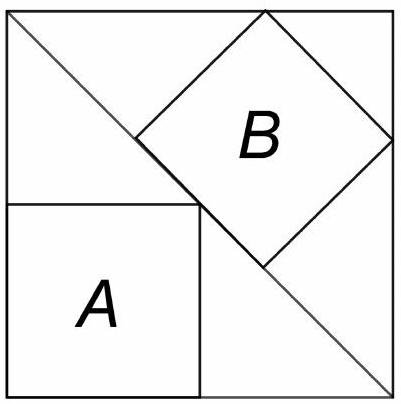
\includegraphics[max width=\textwidth, center]{2024_11_21_a43ce92e94d9b555bf97g-1}


\end{document}